
% Just compile this file using pdflatex after making all required changes.

\documentclass[12pt,a4paper]{report}
\usepackage[pdftex]{graphicx} %for embedding images
\renewcommand{\baselinestretch}{1.5}
%\usepackage{url} %for proper url entries
\usepackage[bookmarks, colorlinks=false, pdfborder={0 0 0}, pdftitle={<pdf title here>}, pdfauthor={<author's name here>}, pdfsubject={<subject here>}, pdfkeywords={<keywords here>}]{hyperref} %for creating links in the pdf version and other additional pdf attributes, no effect on the printed document
%\usepackage[final]{pdfpages} %for embedding another pdf, remove if not required
\usepackage{geometry}
\usepackage[pdftex]{graphicx}
\usepackage{graphicx}
\usepackage{amsmath}
\usepackage{fixltx2e}
\usepackage{multirow}
\usepackage{textcomp}

\geometry{
	left=2.2cm,
	top=2.54cm,
	bottom=2.921cm,
	right=1.5cm
}
\usepackage{fancyhdr}
\pagestyle{fancy}
\lhead{}
\chead{}
\lfoot{\textit{Department of Computer Applications,CET}}
\cfoot{}
\rfoot{\thepage}
\renewcommand{\headrulewidth}{0.4pt}
\renewcommand{\footrulewidth}{0.4pt}
\begin{document}
\renewcommand\bibname{Bibliography} %Renames "Bibliography" to "References" on ref page

%include other pages
\begin{titlepage}
\begin{center}
\textbf{ A  }\\
\vspace{0.35cm}
\textbf{ Seminar Report}\\
\vspace{0.55cm}
\textbf{\Large{A Style-Based Generator Architecture for Generative Adversarial Networks}}\\ \vspace{0.2cm}
\normalsize
\vspace{0.5cm}
\emph{Submitted in partial fulfillment of the requirements for the Award of the Degree}\\
\vspace{0.35cm}
\emph{of}\\
\vspace{0.35cm}
Master of Computer Applications\\
\vspace{0.35cm}
%in\\
%\vspace{0.35cm}
%Computer Science and Engineering(Image processing)\\
%\vspace{0.35cm}
\emph{of}\\
\vspace{0.35cm}
\emph{ {APJ Abdul Kalam Technological University} }\\
\normalsize
\vspace{0.5cm}

\includegraphics[height=0.30\textwidth]{./cet}\\
\vspace{0.3cm}
Submitted by\\
\vspace{0.3cm}
\textbf{VYSHAK PUTHUSSERI}\\
\vspace{0.5cm}
\textbf{RegNo: TVE17MCA054 }\\
\vspace{1.8cm}

\normalsize
\textbf{Department of Computer Applications}\\[0.3cm]
\textbf{COLLEGE OF ENGINEERING TRIVANDRUM}\\[0.4cm]
\textbf{OCTOBER 2019}\\
\end{center}
\end{titlepage}



\begin{titlepage}
\begin{center}
\textbf{DEPARTMENT OF COMPUTER APPLICATIONS}\\[0.5cm]
\textbf{ COLLEGE OF ENGINEERING TRIVANDRUM}\\
[0.5cm]
\vspace{1.2cm}

\includegraphics[width=0.30\textwidth]{./cet}\\
\vspace{0.8cm}
\textbf{CERTIFICATE}\\
%\normalsize
\end{center}
%\normalsize
\emph{Certified that this Seminar report entitled,\textbf{``A Style-Based Generator Architecture for Generative Adversarial Networks"} is the paper presented by \textbf{`` VYSHAK PUTHUSSERI" (Reg No: TVE17MCA054)} in partial fulfillment of the requirements for the award of the degree of Master of Computer Applications of APJ Abdul Kalam Technological University during the year 2019.}\\\\\\\\
\vspace{0.5cm}
Prof. Jose T Joseph.
\hspace{9.5cm}
Prof. Sabitha.\\ 
\hspace{3.9cm} \textbf{Co-ordinator}
\hspace{9.2cm}
%\hspace{0.5cm}
\textbf{Head of the Department}

\end{titlepage}

\begin{titlepage}
\begin{center}
\textbf{\LARGE{Acknowledgement}}\\[0.5cm] 
\end{center}
\paragraph{}
First and for most I thank \textbf{GOD} almighty and to my parents for the success of this seminar. I owe a sincere gratitude and heart full thanks to everyone who shared their precious time and knowledge for the successful completion of my seminar.

I would like to thank \textbf{Dr Jiji C V}, Principal,  College of Engineering Trivandrum, who helped me during the entire process of work.

I am extremely grateful to \textbf{Prof.Sabitha}, HOD, Dept of Computer Applications, for providing me with best facilities and atmosphere for the creative work guidance and encouragement.

I would like to thank my coordinator,\textbf{ Prof.Jose T Joseph}, Dept of Computer Applications, who motivated me throughout the work of my seminar.  

I profusely thank other Asst. Professors in the department and all other staffs of CET, for their guidance and inspirations throughout my course of study.

I owe my thanks to my friends and all others who have directly or indirectly helped me in the successful completion of this seminar. No words can express my humble gratitude to my beloved parents and relatives who have been guiding me in all walks of my journey.\\

 \vspace{1.1cm}
\hspace{345pt} \textbf{Vyshak Puthusseri}


\end{titlepage}

\vspace{2in}
\begin{abstract}
Generative adversarial networks (GANs) is a type of generative model. It is a powerful class of neural networks that are used for unsupervised learning. A GAN consist of two neural networks, a generator network and a discriminator network. The generator generates the data taking random noise as input. The discriminator has to classify whether data generated by the generator is a real or fake data The generator competes against its adversary, the discriminator. As the training for this generative model progresses, the discriminator learns to classify the fake data accurately, while the generator learns to create realistic samples. An equilibrium is reached when the data created by the generator is indistinguishable from real data. GANs are frequently used in image generation and, they produce sharp images too. A downside for GAN is that it does not have a well−defined loss function, which makes training GANs difficult. Although the whole process  was computationally complex as all the possible combinations are tried by the generator to produce realistic data. An alternative generator architecture for GAN was proposed, borrowing from style transfer literature, which reduce the complexity exponentially. The new generator improves the state-of-the-art in terms of traditional distribution quality metrics, leads to demonstrably better interpolation properties. In the end, the result was an  exceptionally differed and excellent dataset of human appearances called FFHQ. The resolution and quality of images produced by generative method using style transfer was of 1024 * 1024, which was exceptionally sufficient include all the human face features. \\\\
Keywords: Generative algorithms, Adversarial training, Style transfer ,Convolutional Neural Network

\end{abstract} 



\pagenumbering{roman} %numbering before main content starts
\tableofcontents
\listoffigures

\newpage
\pagenumbering{arabic} %reset numbering to normal for the main content

    \chapter{Introduction}
\par
The paper coupon market has been with us almost since shopping was first invented. Practically all retail outlets, big or small, have used coupons at least once in their lives. The primary motivation is either to attract more customers by offering them a discount or to enable them to pay in advance for gift vouchers that are subsequently passed on to third parties. The major disadvantage of the paper based coupon was its cost and difficulties in distribution of the coupons. Also the accounting process becomes extremely time consuming. There are issues related to study the market feedback.  A very high proportion of paper coupons are never returned. Paradoxically, a bigger problem is that no firm evidence can be identified to help explain why some actually are returned! All these problems can be solved by digitizing the coupon industry. But a major problem arises due to the arrival of digital coupons. The coupons are getting manipulated by some individuals, which causes a lot of loss to the merchants. So in many situations the loyalty of the customer has to be cross validated by the retailers. 

\par
With the normal encryption mechanism, up to a certain extent this problem can be solved. But if the attacker was highly skilled with tremendous computation power those techniques wont last long. We approach this problem with the disruptive technology, the blockchain. The retailers can generate coupons for a particular product and can share it with the universe using any social media. The coupons are stored in an open source blockchain platform called Ethereum. With the underlying security mechanism of the ethereum blockchain, our system was tamper-proof, as till date nobody was able to break the blockchain network.

    \chapter{Neural Style Transfer}
\begin{styletransfer}
    Style transfer is the technique of recomposing images in the style of other images or we can say style transfer relies on separating the content and style of an image. Given one content image and one style image, we aim to create a new, target image which should contain our desired content and style components:
        \begin{itemize}
            \item objects and their arrangement are similar to that of the content image (feature reconstruction) 
            \item style, colors, and textures are similar to that of the style image (texture synthesis)
        \end{itemize}
     
\section{Content representation and loss}
    We can construct images whose feature maps at a chosen convolution layer match the corresponding feature maps of a given content image. We expect the two images to contain the same content, but not necessarily the same texture and style. Given a chosen content layer \textbf{l}, the content loss is defined as the Mean Squared Error between the feature map \textbf{F} of our content image \textbf{C} and the feature map \textbf{P} of our generated image \textbf{Y}.
    \[Lcontent = \frac{1}{2}\sum_{i j}^{ } \left ( Fij - Pij \right )^{2}\]
    When this content-loss is minimized, it means that the mixed-image has feature activation in the given layers that are very similar to the activation of the content-image. Depending on which layers we select, this should transfer the contours from the content-image to the mixed-image.

\section{Style representation and loss}

    We will do something similar for the style-layers, but now we want to measure which features in the style-layers activate simultaneously for the style-image, and then copy this activation-pattern to the mixed-image. One way of doing this, is to calculate the Gram-matrix(a matrix comprising of correlated features) for the tensors output by the style-layers. The Gram-matrix is essentially just a matrix of dot-products for the vectors of the feature activations of a style-layer.
    If an entry in the Gram-matrix has a value close to zero then it means the two features in the given layer do not activate simultaneously for the given style-image. And vice versa, if an entry in the Gram-matrix has a large value, then it means the two features do activate simultaneously for the given style-image. We will then try and create a mixed-image that replicates this activation pattern of the style-image.If the feature map is a matrix F, then each entry in the Gram matrix G can be given by:
    
   \[ Gij = \sum_{k}^{ } Fik Fjk \]

    The loss function for style is quite similar to out content loss, except that we calculate the Mean Squared Error for the Gram-matrices instead of the raw tensor-outputs from the layers.

    
   \[Lstyle = \frac{1}{2}  \left ( \sum_{i=0}^{L} \left ( Gij - Aij \right )^{2} \right )\]

    As with the content representation, if we had two images whose feature maps at a given layer produced the same Gram matrix we would expect both images to have the same style, but not necessarily the same content. Applying this to early layers in the network would capture some of the finer textures contained within the image whereas applying this to deeper layers would capture more higher-level elements of the image’s style. Gatys et. al [1] found that the best results were achieved by taking a combination of shallow and deep layers as the style representation for an image. The best results are achieved by a combination of many different layers from the network, which capture both the finer textures and the larger elements of the original image.
    \begin{figure}[h]
        \centering
        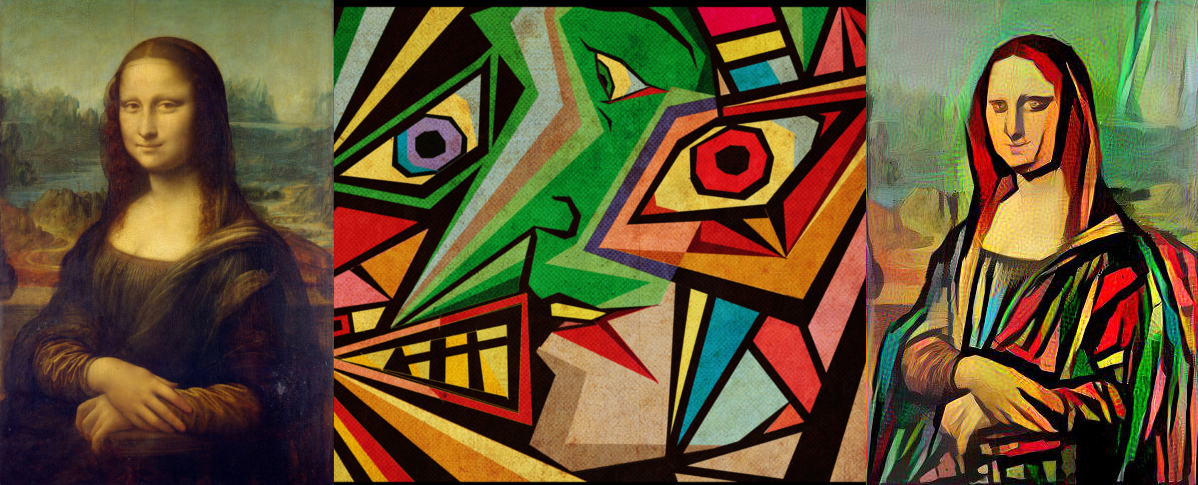
\includegraphics[width=0.8\linewidth]{styletransfer.png}
         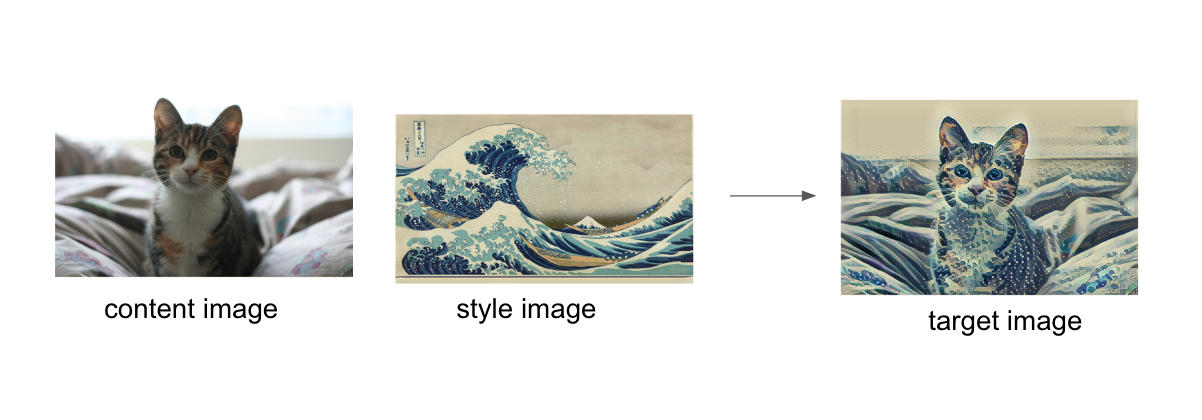
\includegraphics[width=0.8\linewidth]{styletransfercat.png}
        \caption{Style Transfer}
    \end{figure} 

\section{Optimizing loss function and styling the image}
    Using a pre-trained neural network such as VGG-16, an input image (i.e. an image which provides the content), a style image (a painting with strong style elements) and a random image (output image), one could minimize the losses in the network such that the style loss (loss between the output image style and style of ‘style image’), content loss (loss between the content image and the output image) and the total variation loss (which ensured pixel wise smoothness) were at a minimum. In such cases, the output image generated from such a network, resembled the input image and had the stylist attributes of the style image. The total loss can then be written as a weighted sum of the both the style and content losses. 
    \[Ltotal = \alpha Lcontent  + \beta Lstyle \]
    We will minimize our total loss by Adam optimizer. As our loss go down we will go close to our goal of producing a style transfer image Y.

\end{styletransfer}


    \chapter{Generative Adversarial Network}
\begin{onehalfspace}
    A GAN comprises two components, a generator $(G)$ and a discriminator $(D)$. 
    The goal of the generator model is to produce new data similar to the required 
    one. The discriminator's task is to classify the data presented to it as real or 
    fake. Real data belong to the original dataset, and fake data are those 
    forged by the generator. The generative model competes against its adversary, 
    the discriminative model that learns to determine whether a sample is from the 
    model distribution or the data distribution.    
\section{Analogy}
    Generative networks can be thought of as a team of counterfeiters trying 
    to produce fake currency notes and use it without being caught by the 
    police. Here discriminative networks play the role of police trying to 
    detect fake currency. Initially, both the police and counterfeiters are not 
    very experienced, but as the game between them progresses, both parties 
    master what they were doing.  The game continues until the fake currency 
    notes produced by the counterfeiters are indistinguishable from real 
    currency.

\section{A Mathematical Model}

    Assume that the generator represented by the neural network 
    \(G(z, \theta_{1})\) converts the input noise \(z\) into the required output 
    space. Conversely, a second neural network \(D(x, \theta_{2})\) represents 
    discriminator, and it calculates the probability that x came from the real 
    dataset. Here, $\theta_{1}$ and $\theta_{2}$ represents the weights that 
    describe each neural network.

    The discriminator is trained to classify the input data as either real or 
    fake. The weights of the discriminator are updated so that it maximizes the 
    probability that real images from the database are classified as real and 
    minimizes the probability that images generated by G are classified as fake. 
    The loss function used for the discriminator maximizes \(D(x)\) and minimizes 
    \(D(G(z))\). 

    The generator's weights are trained to maximise the probability that it can 
    fool the discriminator using the images it generates. The loss function 
    maximizes \(D(G(z))\).

    \begin{figure}[h]
        \centering
        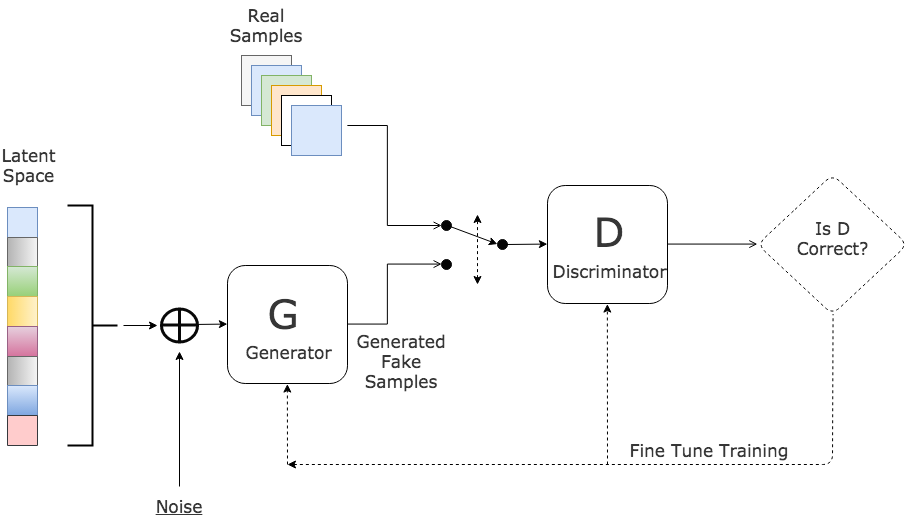
\includegraphics[width=0.8\linewidth]{generative-adversarial-network.png}
        \caption{Generative Adversarial Network Architecture}
        \label{fig:gans}
    \end{figure} 

    Figure \ref{fig:gans} shows a visual representation of the high level 
    overview of GANs discussed in this section.
    During training, the generator is trying to maximize \(D(G(z))\) and 
    discriminator is trying to minimize \(D(G(z))\).  Thus we can think of the 
    scenario as the generator and discriminator as playing a minimax game.
\section{Applications of GAN}
    \subsection{Generate Anime characters}
    Game development and animation production are expensive and hire many production artists for relatively routine tasks. GAN can auto-generate and colorize Anime characters.
    \begin{figure}[h]
        \centering
        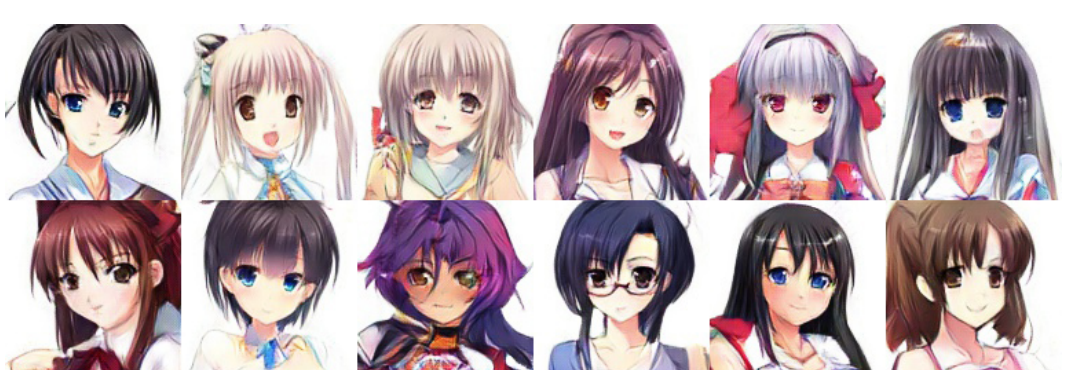
\includegraphics[width=0.8\linewidth]{animecharacter.png}
        \caption{GAN generated anime characters}
    \end{figure} 

    \subsection{CycleGAN}
    Cross-domain transfer GANs will be likely the first batch of commercial applications. These GANs transform images from one domain to another domain.
    (For example, it can transform pictures between zebras and horses.
    \begin{figure}[h]
        \centering
        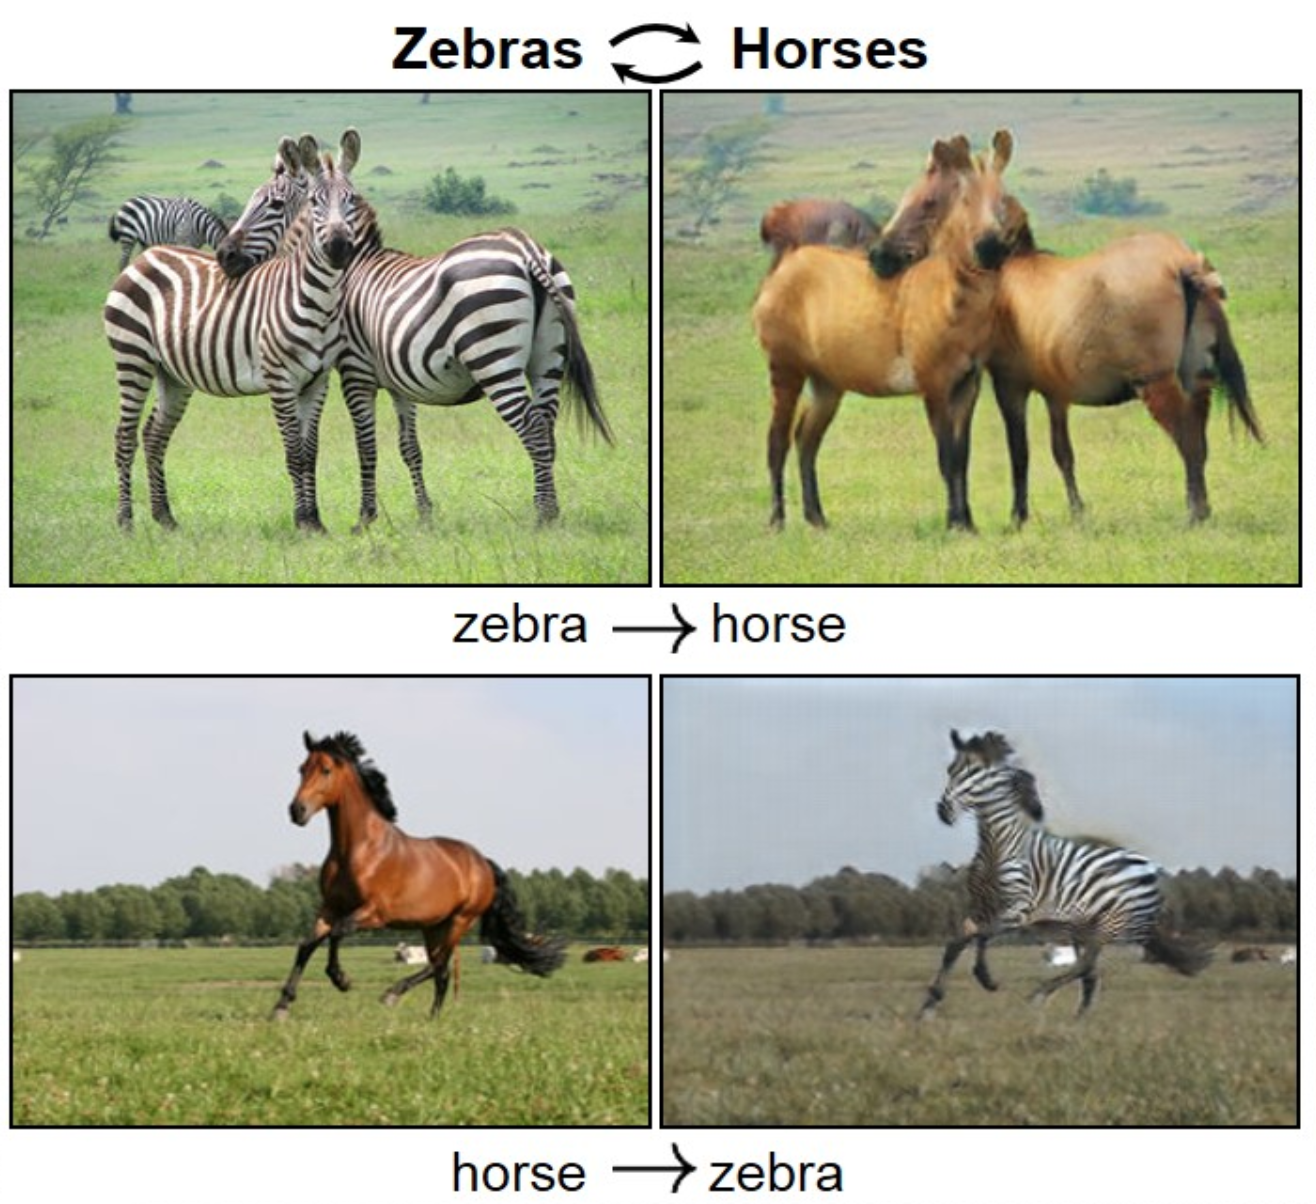
\includegraphics[width=0.5\linewidth]{zebratohorse.png}
        \caption{CycleGAN horse to zebra}
    \end{figure} 
    
    \subsection{PixelDTGAN}
    Suggesting merchandise based on celebrity pictures has been popular for fashion blogger and e-commerce. PixelDTGAN creates clothing images and styles from an image.
    \begin{figure}[h]
        \centering
        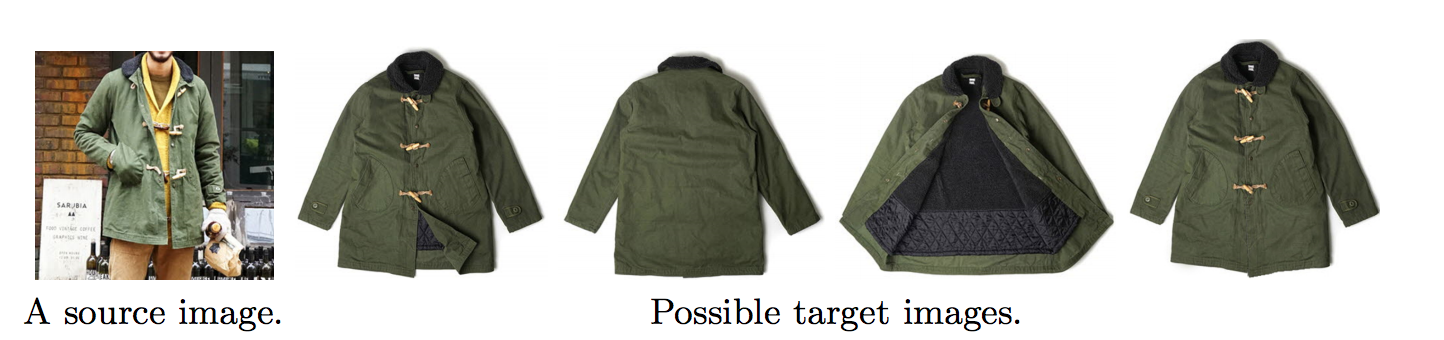
\includegraphics[width=0.5\linewidth]{pixeldtgan.png}
        \caption{PixelDTGAN}
    \end{figure} 
    
    \subsection{Super resolution}
    Create super-resolution images from the lower resolution. This is one area where GAN shows very impressive result with immediate commercial possibility.
    \begin{figure}[h]
        \centering
        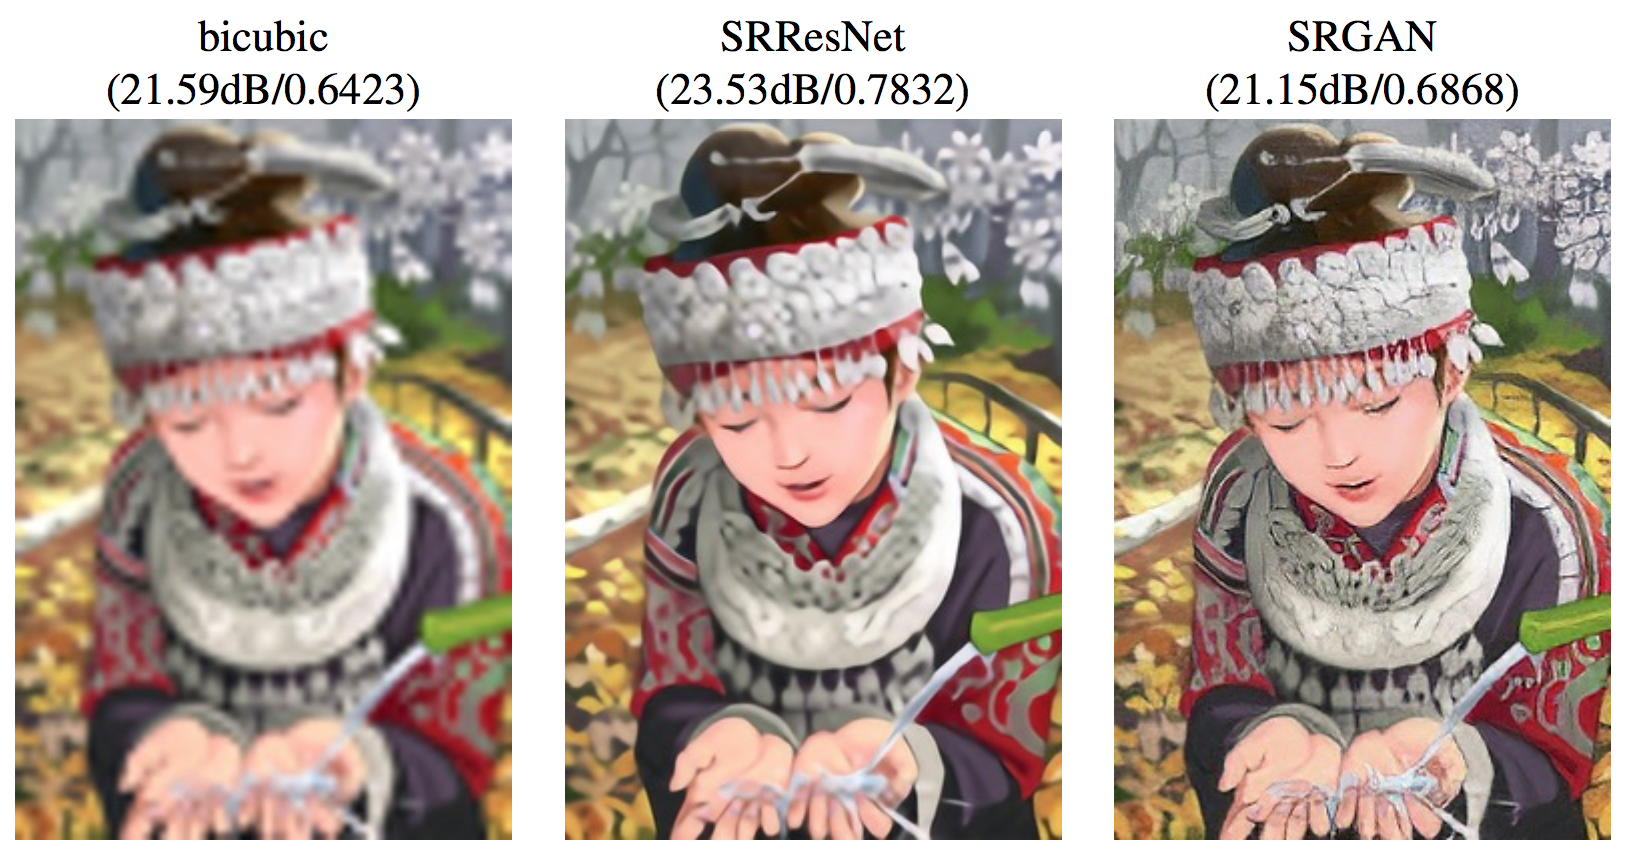
\includegraphics[width=0.5\linewidth]{superresolution.png}
        \caption{SuperResolution using GAN}
    \end{figure} 


\end{onehalfspace}


    \chapter{StyleGAN}
\begin{onehalfspace}
    In past, most improvement has been made to discriminator models in an effort to train more effective generator models, although less effort has been put into improving the generator models. The Style Generative Adversarial Network, or StyleGAN for short, is an extension to the GAN architecture that proposes large changes to the generator model, including the use of a mapping network to map points in latent space to an intermediate latent space, the use of the intermediate latent space to control style at each point in the generator model, and the introduction to noise as a source of variation at each point in the generator model. The resulting model is capable not only of generating impressively photorealistic high-quality photos of faces, but also offers control over the style of the generated image at different levels of detail through varying the style vectors and noise.
\section{Lacking Control Over Synthesized Images}
    Generative adversarial networks are effective at generating high-quality and large-resolution synthetic images. Many improvements to the GAN architecture have been achieved through enhancements to the discriminator model. These changes are motivated by the idea that a better discriminator model will, in turn, lead to the generation of more realistic synthetic images. As such, the generator has been somewhat neglected and remains a black box. This limited understanding of the generator is perhaps most exemplified by the general lack of control over the generated images. There are few tools to control the properties of generated images, e.g. the style. This includes high-level features such as background and foreground, and fine-grained details such as the features of synthesized objects or subjects.


\section{Control Style Using New Generator Model}

   The Style Generative Adversarial Network, or StyleGAN for short, is an extension to the GAN architecture to give control over the disentangled style properties of generated images. The StyleGAN is an extension of the progressive growing GAN that is an approach for training generator models capable of synthesizing very large high-quality images via the incremental expansion of both discriminator and generator models from small to large images during the training process. In addition to the incremental growth of the models during training, the style GAN changes the architecture of the generator significantly. The StyleGAN generator no longer takes a point from the latent space as input; instead, there are two new sources of randomness used to generate a synthetic image: a standalone mapping network and noise layers. The output from the mapping network is a vector that defines the styles that is integrated at each point in the generator model via a new layer called adaptive instance normalization. The use of this style vector gives control over the style of the generated image. Stochastic variation is introduced through noise added at each point in the generator model. The noise is added to entire feature maps that allow the model to interpret the style in a fine-grained, per-pixel manner. This per-block incorporation of style vector and noise allows each block to localize both the interpretation of style and the stochastic variation to a given level of detail.
\section{Architecture}
The StyleGAN is described as a progressive growing GAN architecture with five modifications, each of which was added and evaluated incrementally in an ablative study.
The incremental list of changes to the generator are:
    \begin{itemize}
        \item Baseline Progressive GAN.
        \item Addition of tuning and bilinear upsampling.
        \item Addition of mapping network and AdaIN (styles).
        \item Addition of noise to each block.
        \item Addition Mixing regularization.
    \end{itemize}
    \begin{figure}[h]
        \centering
        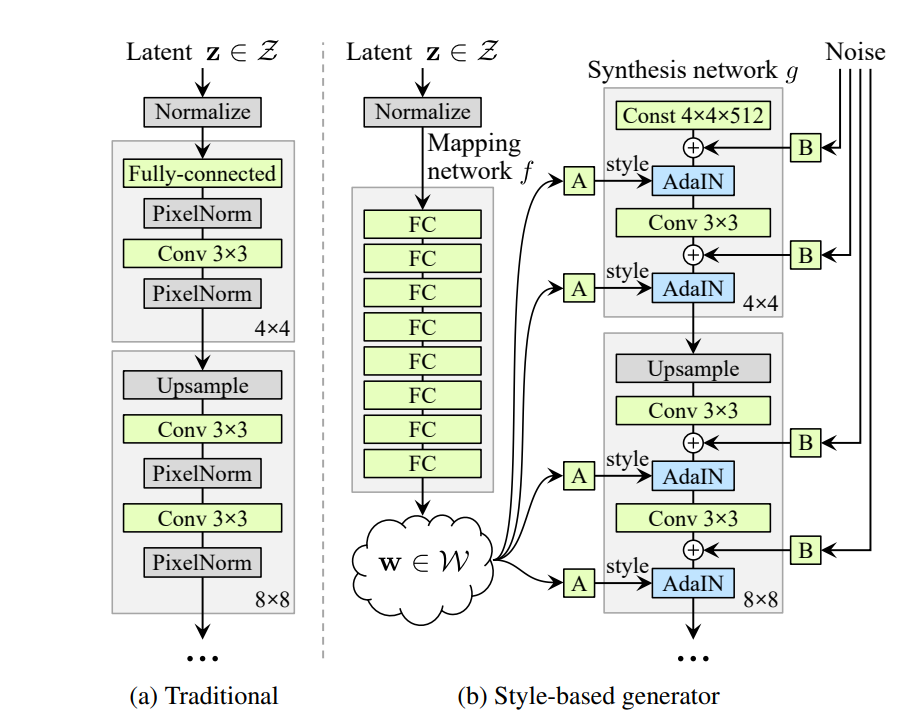
\includegraphics[width=0.8\linewidth]{styleganarchitecture.png}
        \caption{Style GAN Architecture}
    \end{figure} 
    \subsection{Baseline Progressive GAN}
    The StyleGAN generator and discriminator models are trained using the progressive growing GAN training method. This means that both models start with small images, in this case, 4×4 images. The models are fit until stable, then both discriminator and generator are expanded to double the width and height (quadruple the area), e.g. 8×8. A new block is added to each model to support the larger image size, which is faded in slowly over training. Once faded-in, the models are again trained until reasonably stable and the process is repeated with ever-larger image sizes until the desired target image size is met, such as 1024×1024.
    
    \subsection{Bilinear Sampling}
    The progressive growing GAN uses nearest neighbor layers for upsampling instead of transpose convolutional layers that are common in other generator models. The first point of deviation in the StyleGAN is that bilinear upsampling layers are unused instead of nearest neighbor.

    \subsection{Mapping Network and AdaIN}
    Next, a standalone mapping network is used that takes a randomly sampled point from the latent space as input and generates a style vector. The mapping network is comprised of eight fully connected layers. The style vector is then transformed and incorporated into each block of the generator model after the convolutional layers via an operation called adaptive instance normalization or AdaIN. The AdaIN layers involve first standardizing the output of feature map to a standard Gaussian, then adding the style vector as a bias term. The addition of the new mapping network to the architecture also results in the renaming of the generator model to a “synthesis network.”

    
    \subsection{Addition of Noise}
    The output of each convolutional layer in the synthesis network is a block of activation maps. Gaussian noise is added to each of these activation maps prior to the AdaIN operations. A different sample of noise is generated for each block and is interpreted using per-layer scaling factors. This noise is used to introduce style-level variation at a given level of detail.


    \subsection{Mixing regularization}
    Mixing regularization involves first generating two style vectors from the mapping network. A split point in the synthesis network is chosen and all AdaIN operations prior to the split point use the first style vector and all AdaIN operations after the split point get the second style vector. This encourages the layers and blocks to localize the style to specific parts of the model and corresponding level of detail in the generated image.




\end{onehalfspace}


    \chapter{Conclusion}

\par
The retailers create a promo code for a particular product with some
discount and add the corresponding details get added into the blockchain.
Corresponding to the data added, a hash value gets generated. Using the hash
value, a QR code is going to be generated, and which is going to be publicly
advertise. The customer with that QR code can go to a verified dealer and he
can give the discount as prescribed. Till date no one was able to tamper the
blockchain technology and so our system.
The system provides permanent solution for the customer locality problem, makes it easily accessible from anywhere and everywhere. Cryptography protection ensures that the data is tamper-proof and immutable. The digital coupons help us to avoid the delay in physically doing the transactions. Moreover, it can help us to save time. It solves all such problems of traditional coupon industry. The implementation of this system will mop off fake coupons generation and manipulations. 


%%%%%%%%%%%%%%%%%%%%%%%% Bibilography

\begin{thebibliography}{9}
\bibitem{styletransfer} 
L. A. Gatys, A. S. Ecker, and M. Bethge.
\textit{ Image style transfer using convolutional neural networks.}
In Proc. CVPR, 2016.
 
\bibitem{GAN} 
I.Goodfellow, J.Pouget-Abadie, M.Mirza, B.Xu, D.Warde-Farley, S. Ozair, A.Courville, and Y.Bengio. 
\textit{ Generative Adversarial Networks.} In NIPS, 2014.
 
\bibitem{ADAM} 
D. P. Kingma and Jimmy Ba.
\textit{ Adam: A method for stochastic optimization.}  In ICLR, 2015.

\bibitem{backpropogation} 
D. J. Rezende, S. Mohamed, and D. Wierstra.
\textit{  Stochastic backpropagation and approximate inference in deep generative models.} In Proc. ICML, 2014

\bibitem{improved gan} 
T. Salimans, I. J. Goodfellow, W. Zaremba, V. Cheung, A. Radford, and X. Chen.
\textit{  Improved techniques for training GANs.}In NIPS, 2016.

\bibitem{avoid overfitting} 
N. Srivastava, G. Hinton, A. Krizhevsky, I. Sutskever, and R. Salakhutdinov.
\textit{  Dropout: A simple way to prevent neural networks from overfitting.}  Journal of Machine Learning Research, 15:1929–1958, 2014



\end{thebibliography}



\end{document}
